
 \section{Diseñe la gramática del lenguaje de programación propuesto. Puede basarse de ejemplos que hay internet.}
 \subsection{Tokens}
\begin{center}
    \resizebox{9cm}{!} {
    \begin{tabular}{r l}
    
    ID ::=  &'[a-zA-Z]+ ([a-zA-Z0-9]*)'\\
    PLUS ::= &'+'\\
    MINUS ::= &'-'\\
    MULTI ::= &'*'\\
    DIVIDE ::= &'/'\\
    ASSIGNMENT ::= &'=' \\
    EQUALITY ::= &'=='\\
    SUM_ASSIGNMENT ::= &'+='\\
    REST_ASSIGNMENT ::= &'-='\\
    LPAREN ::= &'('\\
    RPAREN ::= &')'\\
    LSB ::= &'['\\
    RSB ::= &']'\\
    LB ::= &'\{'\\
    RB ::= &'\}'\\
    GREATER ::= &'>'\\  
    MINOR ::= &'<'  \\
    GREATER_EQUAL ::= &'>='\\  
    MINORE_QUAL ::= &'<='\\
    AND ::= &'y'\\
    OR ::= &'o'\\
    DISTINCT ::= &'!='\\
    PERCENT ::= & '\%' \\
    EXCLAM ::=&  '!'\\
    \end{tabular}
    }
\end{center}

 \subsection{Palabras reservadas:}

\begin{center}
    \resizebox{5.5cm}{!} {
    \begin{tabular}{r l}
        IF ::= 'si' \\
        ELSE ::= &'sino'\\
        FOR ::= &'para'\\
        WHILE ::= &'mientras'\\
        BREAK ::= &'romper'\\ 
        FUNCTION ::= &'funcion'\\
        RETURN ::= &'returnar'\\
        VAR ::= &'variable'\\
        CONST ::= &'constante'\\    
        LET ::= &'temporal'\\
        TRUE ::= &'verdadero'\\
        FALSE ::= &'falso'\\
        FALSE ::= &'falso'\\
        CONSOLE.LOG ::= & 'imprimir' \\
        
      
    \end{tabular}
    }
\end{center}
        
        
        
        
        
        
        
        
        
\subsection{Inicio programa}

\begin{verbatim}
    Programa ::= Declaracion | Expresion
\end{verbatim}

\subsection{Expresiones:}

\begin{verbatim}
    Expresion ::= &Expresion (Y 
                     | O             | GREATER   | MINOR         | PLUS 
                     | MINUS         | MULTI     | DIVIDE        | MINORE_QUAL 
                     | GREATER_EQUAL | EQUALITY  | PERCENT       | DISTINCT ) Expression  
             | "verdadero"  
             | "falso"       | "!" ID 
             | (Expresion)   | ID 
    

\end{verbatim}

\subsection{Declaraciones:}
\begin{verbatim}
    Declaracion	::=	LB LPAREN Declaracion RPAREN RB
                    | CONSOLE.LOG LPAREN ((ID ,)* ID)+ RPAREN 
            	    | IF LPAREN Expresion RPAREN
            	    | IF LPAREN Expresion RPAREN Declaracion
            	    | IF LPAREN Expresion RPAREN Declaracion ELSE Declaracion
            	    | FOR LPAREN Expresion RPAREN Expresion Expresion RPAREN Declaracion
            	    | WHILE LPAREN Expresion RPAREN Declaracion
            	    | FUNCTION ID LPAREN ((ID ,)* ID)+ RPAREN LB Expresion RETURN Expresion RB
\end{verbatim}

\subsection{Tipos:}

\begin{verbatim}
    Tipo ::=  ("entero" | "decimal" | "booleano" | "caracter" | ) Identificador
\end{verbatim}

\subsection{Haciendo pruebas de entrada}
El codigo que probaremos será el siguiente
\begin{verbatim}
constante var1 = 10 + 10
\end{verbatim}
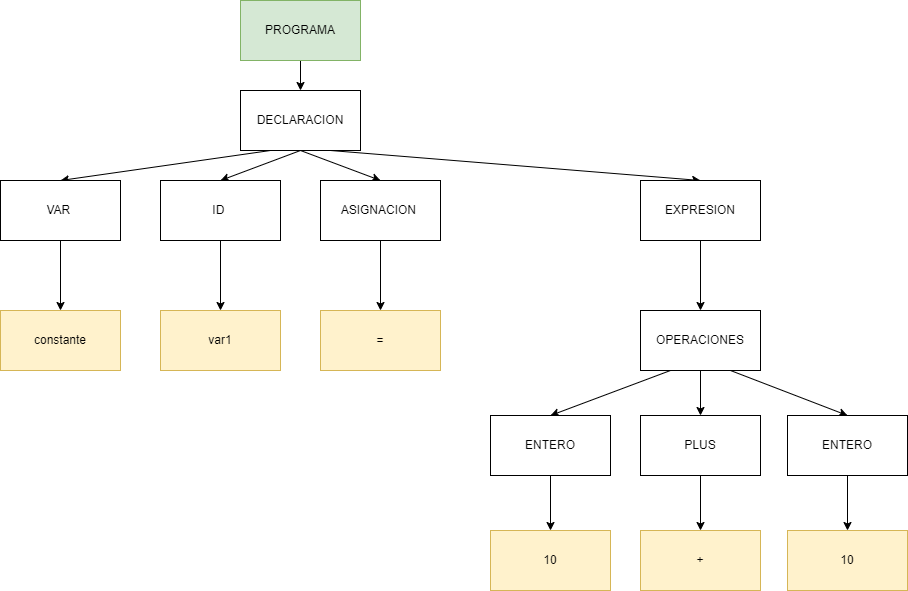
\includegraphics[width=15cm]{images/arbol.png}


